\chapter{Theoretical Performance Evaluation and Comparison against Roofline Model}
\label{sec:theory_performance}
% formalize model!!!
% T_comm = (2r(t_w+t_h) * 4 \text{ bytes}) / (\text{Bandwidth_per_link})
% T_comp = (t_w * t_h * (4r+1) * \text{cycles_per_fmac}) / s_simd
% Pessimistic: T_total = T_comp + T_comm
% Optimistic: T_total = max(T_comp, T_comm) (assuming perfect overlap)



update plot!
actual roofline plot ???

In this section the theoretical best performance of the implemented algorithms given the Cerebras hardware constraints is analyzed.
We assume the data type to be float32 throughout this section.
We find that the cycle count for one stencil iteration is limited by following factors:
\begin{itemize}
    \item Communication time ($T_{comm}$), i.e. the total amount of data send and received divided by link throughput
    \item Computation time ($T_{comp}$), i.e. total amount of computation divided by peak performance
    \item Communication delay ($T_{delay}$), i.e. total amount of time spent waiting for data while no computation can be done
\end{itemize}

An optimistic estimate for the total achivable cycle count assumes perfect overlap between the three limiting factors, while a pessimistic estimate assumes no overlap.



\section{Radius 1, no tiling}
The \ac{ce} must receive the values from its four neighbors. Since the link capacity between the router and \ac{ce} is 32 bit per cycle, this will take four cycles in the best case.

The received data can immediately be used for computation as the \texttt{@fadds} and \texttt{@fmacs} commands can use dsds of type \texttt{fabin\_dsd} as an input. This means most of the computation can be done during the receiving of the data. Only one extra cycle is necessary to take into account the old $value$. With a clever implementation this extra computation could be executed during the communication delay idle time so that it doesn't affect the overall cycle count.

Sending takes one cycle from \ac{ce} to its router, another cycle from the router to its neighbors routers and a third cycle from these routers to the neighbors \acp{ce}. This results in three cycles for the communication delay.

In total this results in seven cycles per stencil operation that could be achieved in theory.
Note that this is independent of the actual grid size (as long as it fits onto the \ac{wse}).

\section{Any radius and tiling}
Similarly to before the total computation for one iteration can be split up into the same three fundamental steps. We now need to take the radius $r$, tile width $t_w$ and tile height $t_h$ into account.

Each \ac{pe} needs data from its four neighbors. $r\cdot t_w$ elements from the northern and southern neighbors and $r\cdot t_h$ elements from the western and eastern neighbors. This results in $2r(t_w+t_h)$ total elements and cycles for data receiving.

During the computation $4r+1$ multiply-add operations per grid element are required which results in $t_wt_h(4r+1)$ multiply-add operations per \ac{pe}. With SIMD execution we can parallelize this and divide it by the SIMD width for \texttt{@famcs} which is 4 on wse-2 and 8 on wse-3. This results in $\left\lceil\frac{t_wt_h(4r+1)}{s}\right\rceil$. This term exceeds the communication term for most parameter combinations of $t_w,\ t_h$ and $r$. Assuming the first part of the computation could still be done during communication, we can drop the communication term completely. Note that this is a rather optimistic assumption and likely not achievable with the hardware.

The communication delay is in this case negligible and could be overlapped with the computation in a way that it doesn't affect the cycle count. 

This results in a total cycle count of $\left\lceil\frac{t_wt_h(4r+1)}{s}\right\rceil$ which is just the computation time and assuming we can fully overlap the communication time as an optimistic estimate. As a slightly pessimistic estimate we get $\left\lceil\frac{t_wt_h(4r+1)}{s}\right\rceil+2r(t_w+t_h)$ which assumes no possible overlap between communication and computation. 

It becomes clear that for radius 1 the tiled stencil gets significantly slower than the non-tiled implementation. 
\begin{figure}
    \centering
    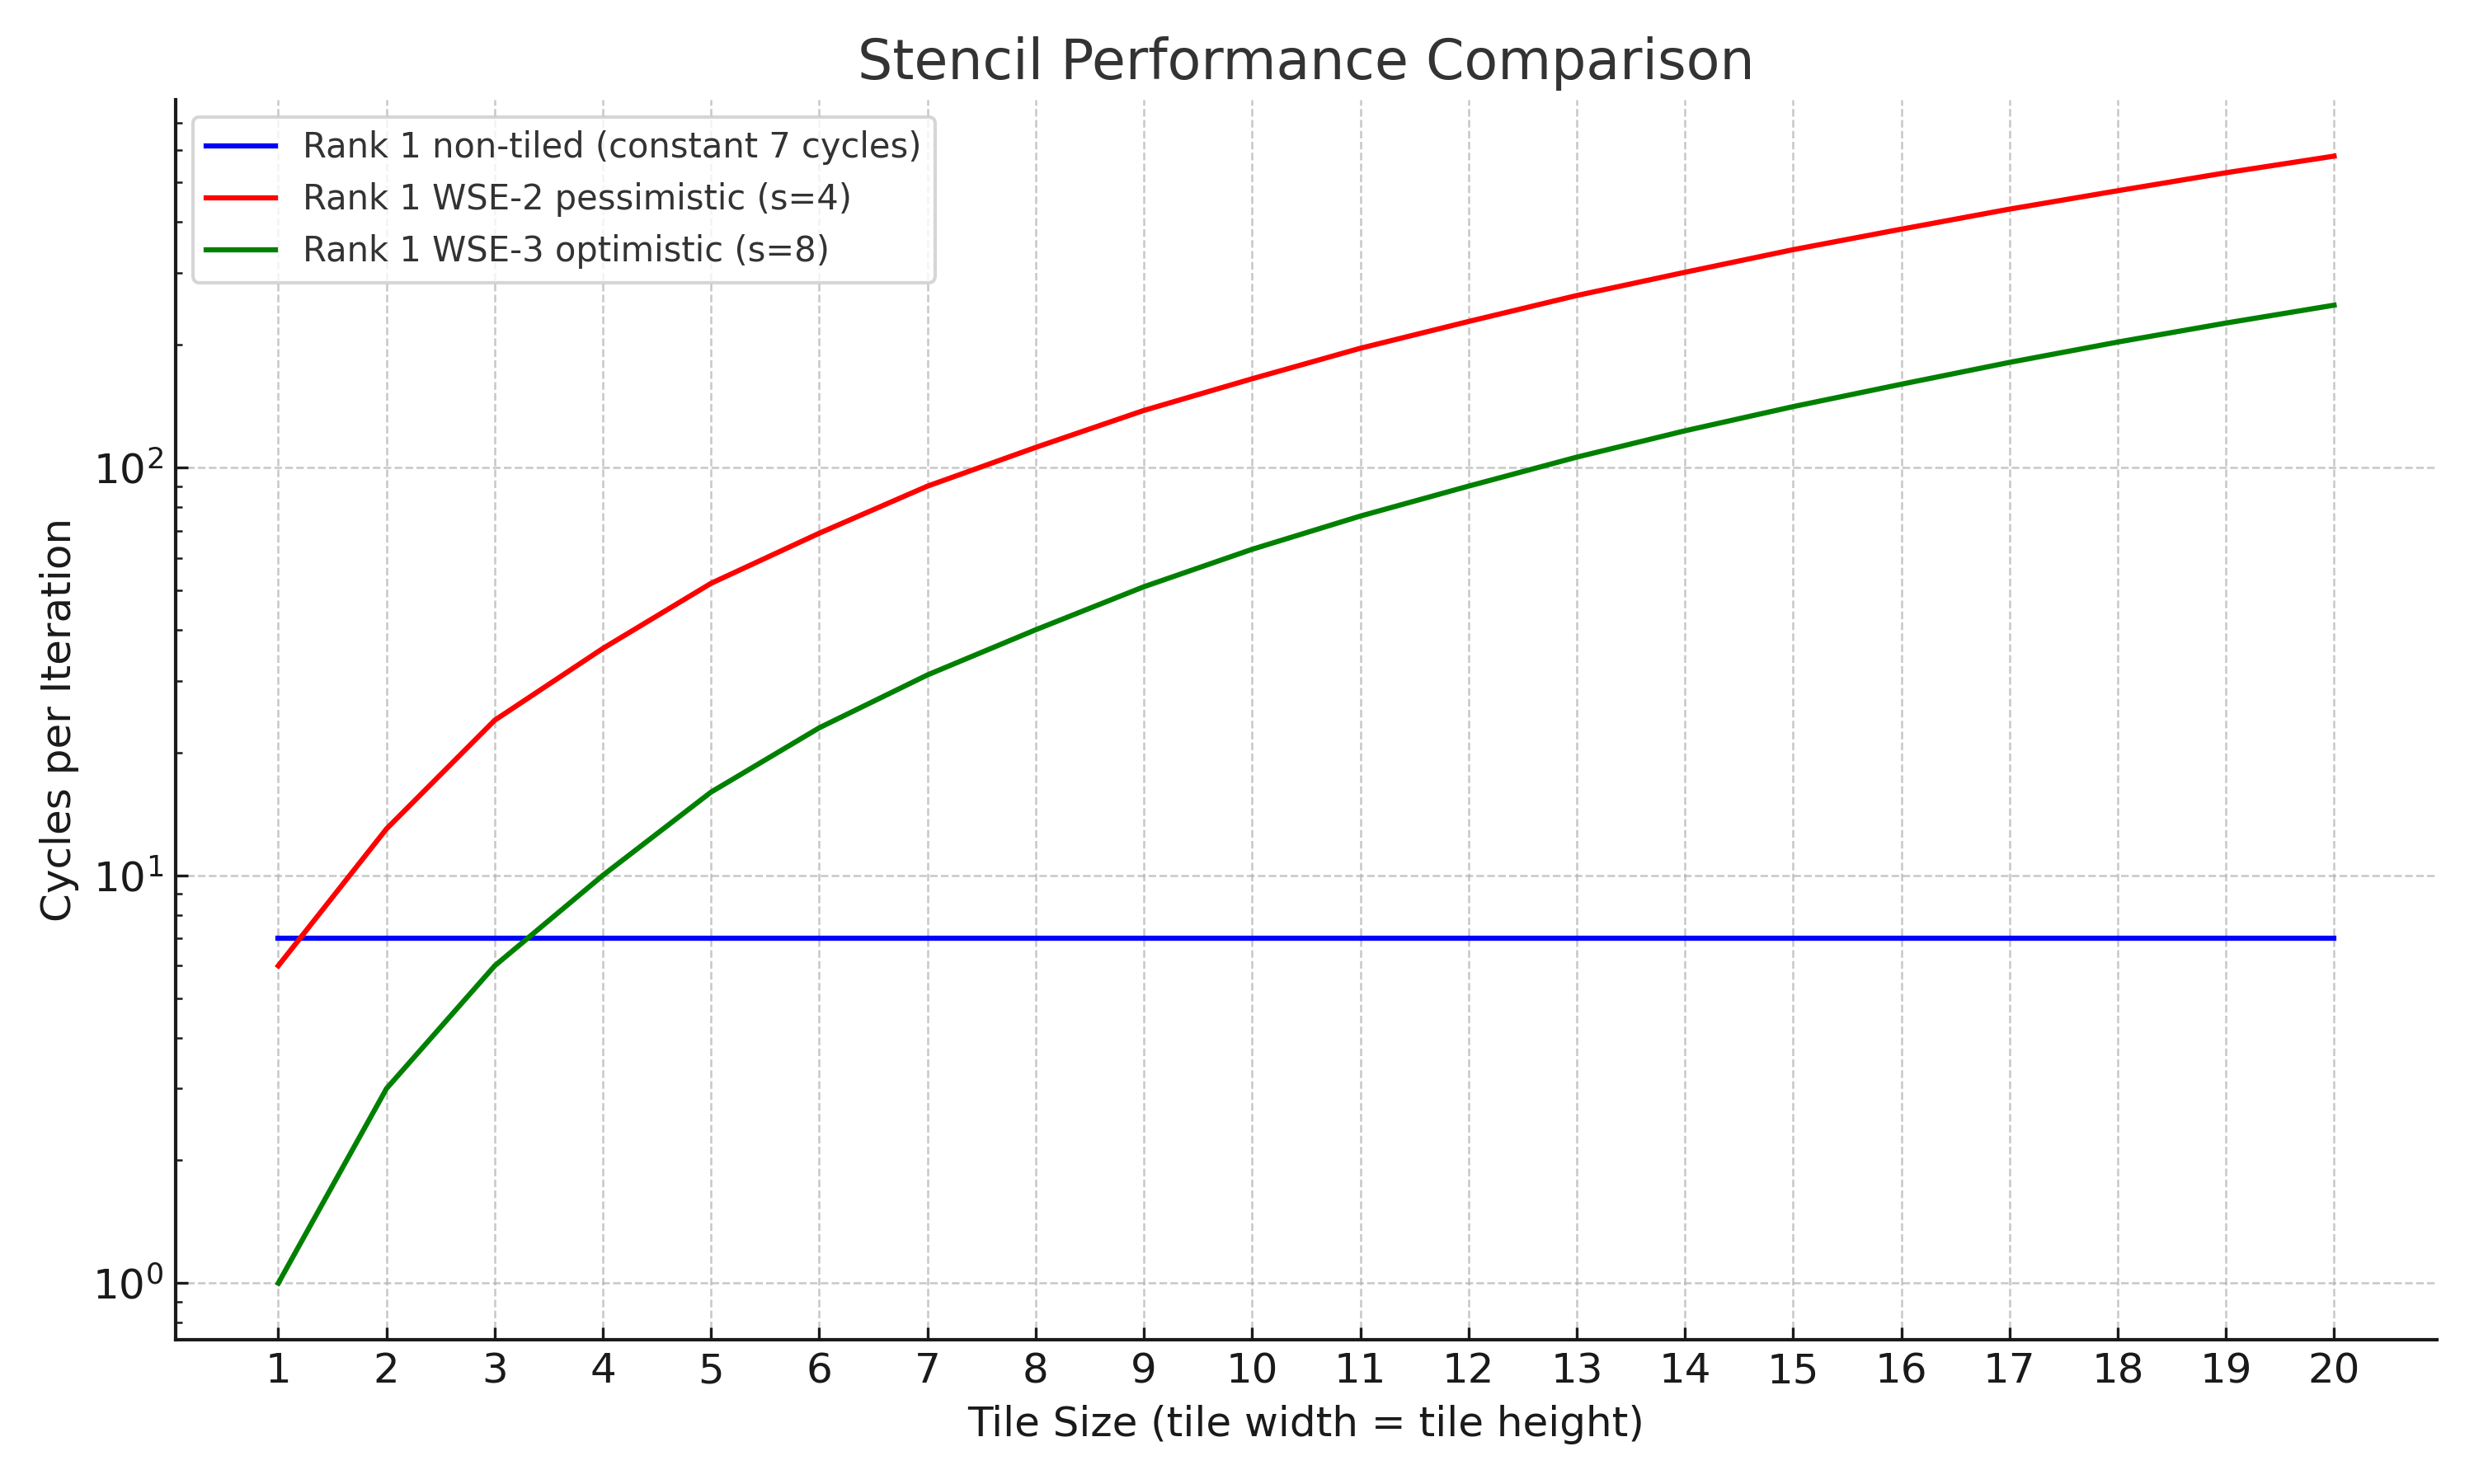
\includegraphics[width=0.5\linewidth]{stencil_performance_comparison.png}
    \caption{Cycles per iteration for tiled and non-tiled stencils theoretical performance with radius 1}
    \label{fig:enter-label}
\end{figure} 